% Source: Wald GR, physical PDF pp. 149--160
%         (printed pp. 136--147).
% Coverage: Section 6.3, Geodesics of Schwarzschild: Gravitational Redshift,
%           Perihelion Precession, Bending of Light, and Time Delay of Radar
%           Signals; equations (6.3.1)--(6.3.47).
% Figures/tables/footnotes: Figs. 6.2--6.7; no tables or footnotes.
% Status: source-reviewed and compile-clean.
% Uncertainties: none.

\subsection{Geodesics of Schwarzschild: Gravitational Redshift, Perihelion
Precession, Bending of Light, and Time Delay of Radar Signals}\label{sec:6.3}

In this section, we will analyze the behavior of test bodies and light rays in
the exterior region (\(r>2M\)) of the Schwarzschild solution by solving for the
timelike and null geodesics of the Schwarzschild geometry. Our analysis of the
geodesics in the strong field regime (\(r\) near \(2M\)) is physically relevant,
of course, only for highly condensed stars or totally collapsed objects, but our
results in the weak field regime (\(r\gg M\)) apply to the exterior field of
ordinary bodies such as the Sun.

It would involve a fair amount of labor to solve directly the geodesic equation
in the form Eq.~\eqref{eq:3.3.5}. Fortunately, almost all of this labor can be
avoided by taking advantage of the symmetries of the Schwarzschild solution using
proposition C.3.1 of appendix C: The inner product, \(u^a\xi_a\), of a Killing
field \(\xi^a\) with a geodesic tangent \(u^a\) is constant along the geodesic. As
we shall see below, these constants of the motion enable us to reduce the problem
of finding the geodesics to the problem of one-dimensional motion of a particle in
an effective potential.

Proposition C.3.1 immediately allows us to derive a formula for the change between
emitted and observed frequency of light signals sent between two static observers,
i.e., for the gravitational redshift. (A similar derivation of the cosmological
redshift in an expanding homogeneous and isotropic universe was given above in
Section~5.3a.) Consider two static observers, i.e., observers whose 4-velocity is
tangent to the static Killing field \(\xi^a\), \(O_1\) and \(O_2\), whose
4-velocities are \(u_1^a\) and \(u_2^a\). Suppose \(O_1\) emits a light signal at
event \(P_1\) which is received by \(O_2\) at event \(P_2\), as illustrated in
Figure~\ref{fig:6.2}. As discussed in Section~4.3, in the geometrical optics
approximation this light signal travels on a null geodesic, whose tangent we
denote by \(k^a\).
% Source: Wald GR, physical PDF p. 149
%         (printed p. 136).
% Coverage: Figure 6.2, a light signal sent by a static observer.
% Figures/tables/footnotes: Figure 6.2; no tables or footnotes.
% Status: source-reviewed and compile-clean.
% Uncertainties: none.
\begingroup
\renewcommand{\thefigure}{6.2}
\begin{figure}[htbp]
\centering
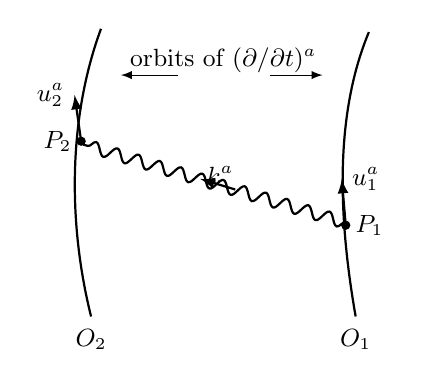
\begin{tikzpicture}[scale=.84,>=latex,font=\small]
  \draw[thick] (-2.0,-2.2) .. controls (-2.35,-.8) and (-2.35,.8) .. (-1.85,2.15);
  \draw[thick] (2.0,-2.2) .. controls (1.72,-.6) and (1.70,.9) .. (2.20,2.1);
  \fill (-2.15,.45) circle (2pt) node[left] {\(P_2\)};
  \fill (1.85,-.82) circle (2pt) node[right] {\(P_1\)};
  \draw[->,thick] (-2.15,.45) -- (-2.25,1.15) node[left] {\(u_2^a\)};
  \draw[->,thick] (1.85,-.82) -- (1.79,-.12) node[right] {\(u_1^a\)};
  \draw[thick,decorate,decoration={snake,amplitude=2.2pt,segment length=8pt}]
    (1.84,-.78) -- (-2.12,.40);
  \draw[->,thick] (.18,-.28) -- (-.35,-.12);
  \node at (-.05,-.07) {\(k^a\)};
  \draw[->] (-.68,1.45) -- (-1.55,1.45);
  \draw[->] (.70,1.45) -- (1.50,1.45);
  \node at (0,1.67) {orbits of \((\partial/\partial t)^a\)};
  \node at (-2.0,-2.55) {\(O_2\)};
  \node at (2.0,-2.55) {\(O_1\)};
\end{tikzpicture}
\caption{A spacetime diagram showing a light signal sent from static observer
\(O_1\) to static observer \(O_2\).}
\label{fig:6.2}
\end{figure}
\endgroup

The frequency of emission is
\begin{equation}
  \omega_1=-\left.(k_au_1^a)\right|_{P_1},
  \tag{6.3.1}\label{eq:6.3.1}
\end{equation}
while the frequency measured by the observer receiving the signal is
\begin{equation}
  \omega_2=-\left.(k_au_2^a)\right|_{P_2}.
  \tag{6.3.2}\label{eq:6.3.2}
\end{equation}
However, since \(u_1^a\) and \(u_2^a\) both are unit vectors which point in the
direction of the timelike Killing field \(\xi^a\), we have
\begin{align}
  u_1^a&=\left.\left[\frac{\xi^a}{(-\xi^b\xi_b)^{1/2}}\right]\right|_{P_1},
  &&\tag{6.3.3}\label{eq:6.3.3}\\
  u_2^a&=\left.\left[\frac{\xi^a}{(-\xi^b\xi_b)^{1/2}}\right]\right|_{P_2}.
  &&\tag{6.3.4}\label{eq:6.3.4}
\end{align}
By proposition C.3.1 we have
\(\left.(k_a\xi^a)\right|_{P_1}=\left.(k_a\xi^a)\right|_{P_2}\), so we obtain
\begin{equation}
  \frac{\omega_1}{\omega_2}
  =\frac{\left.(-\xi^b\xi_b)^{1/2}\right|_{P_2}}
         {\left.(-\xi^b\xi_b)^{1/2}\right|_{P_1}}
  =\frac{(1-2M/r_2)^{1/2}}{(1-2M/r_1)^{1/2}},
  \tag{6.3.5}\label{eq:6.3.5}
\end{equation}
where the explicit form of \(\xi^b\xi_b=g_{tt}=-(1-2M/r)\) for Schwarzschild
spacetime has been used and \(r_1\) and \(r_2\) are, respectively, the radial
coordinates of \(O_1\) and \(O_2\). Note, however, that the above derivation is
valid in an arbitrary stationary spacetime.

Equation~\eqref{eq:6.3.5} shows that for \(r_2>r_1\), i.e., for the emitter
closer to the center of gravitational attraction than the receiver, we have
\(\omega_2<\omega_1\), i.e., the frequency of the light will be decreased
(shifted toward the red). Physically, this makes sense because according to
quantum theory the energy of a photon is proportional to its frequency,
\(E=\hbar\omega\), and we would expect the photon energy to be degraded as it
climbs out of the gravitational potential well. Indeed, in the limit where \(M\)
is much less than \(r_1\) and \(r_2\), as is the case outside the surface of
ordinary bodies, Eq.~\eqref{eq:6.3.5} becomes
\begin{equation}
  \frac{\Delta\omega}{\omega}\approx-\frac{GM}{c^2r_1}
  +\frac{GM}{c^2r_2},
  \tag{6.3.6}\label{eq:6.3.6}
\end{equation}
where we have restored the \(G\)'s and \(c\)'s in this equation. This can be
interpreted as saying that the change in the locally measured energy of a photon,
\(\hbar\Delta\omega\), equals the change in its Newtonian gravitational potential
energy \((\hbar\omega/c^2)(-GM/r_1+GM/r_2)\).

The gravitational redshift has been measured and found to be in agreement with the
prediction of general relativity to within the \(1\%\) experimental uncertainty by
a laboratory experiment devised by Pound and Rebka (1960) which uses the
M\"ossbauer effect to measure the tiny frequency shift of photons on the surface
of the Earth which fall down a tower. The gravitational redshift of spectral lines
from the Sun and some white dwarf stars has also been observed, but the accuracy of
these measurements for testing Eq.~\eqref{eq:6.3.5} is not as high due to
convective motions (which broaden the spectral lines) in the case of the Sun and a
number of other uncertainties in the case of the white dwarfs. More recently, the
gravitational redshift has been confirmed to about \(0.01\%\) accuracy by the
tracking of hydrogen masers launched by rocket (Vessot and Levine 1979; Vessot
\emph{et al.}\ 1980). Confirmation of the existence of a similar gravitational
time dilation effect also has been achieved by comparison of atomic clocks flown
in airplanes with clocks on the ground (Hafele and Keating 1972; Alley 1979).

It is worth pointing out that, as proven in Section~\ref{sec:6.2}, the maximum
value of \(M/R\) at the surface of a static spherical body (with
\(d\rho/dr\leq0\) everywhere inside the body) is \(4/9\). Thus, by
Eq.~\eqref{eq:6.3.5}, the maximum redshift of light emitted from the surface of a
static star is
\begin{equation}
  \left.\frac{\omega_1}{\omega_2}\right|_{\max}
  =\frac{\omega(r=9M/4)}{\omega(r=\infty)}=3,
  \tag{6.3.7}\label{eq:6.3.7}
\end{equation}
i.e., in terms of the redshift factor \(z\) defined in Chapter~5, we have
\begin{equation}
  z_{\max}=\left.\frac{\omega_1}{\omega_2}\right|_{\max}-1=2.
  \tag{6.3.8}\label{eq:6.3.8}
\end{equation}
This rules out the possibility that observed redshifts of greater than 2 (as are
commonly found for quasars) could arise solely from the gravitational redshift of
light emitted from the surface of a static, spherical body.

In order to learn more about the behavior of light rays and test bodies in the
exterior gravitational field of a spherical body, we need to solve for the
timelike and null geodesics. First, we note that because of the parity reflection
symmetry \(\theta\mapsto\pi-\theta\) of the Schwarzschild metric, if the initial
position and tangent vector of a geodesic lie in the equatorial plane
\(\theta=\pi/2\), then the entire geodesic must lie in this plane. Since every
geodesic can be brought to an initially (and hence everywhere) equatorial
geodesic by a rotational isometry, this means that without loss of generality we
may restrict attention to study of the equatorial geodesics, and we shall do so.
The coordinate basis components of the tangent \(u^a\) to a curve parametrized by
\(\tau\) are (see Eq.~\eqref{eq:2.2.12})
\begin{equation}
  u^\mu=\frac{dx^\mu}{d\tau}\equiv\dot x^\mu.
  \tag{6.3.9}\label{eq:6.3.9}
\end{equation}
For timelike geodesics, we choose \(\tau\) to be the proper time; and for null
geodesics, we choose \(\tau\) to be an affine parameter. Thus for these cases we
have (recalling that \(\theta=\pi/2\))
\begin{equation}
  -\kappa=g_{ab}u^au^b
  =-(1-2M/r)\dot t^2+(1-2M/r)^{-1}\dot r^2+r^2\dot\phi^2,
  \tag{6.3.10}\label{eq:6.3.10}
\end{equation}
where
\begin{equation}
  \kappa=
  \begin{cases}
    1 & \text{(timelike geodesics)},\\
    0 & \text{(null geodesics)}.
  \end{cases}
  \tag{6.3.11}\label{eq:6.3.11}
\end{equation}

In the derivation of the gravitational redshift, we already used the fact that
the quantity
\begin{equation}
  E=-g_{ab}\xi^au^b=(1-2M/r)\dot t
  \tag{6.3.12}\label{eq:6.3.12}
\end{equation}
is a constant of the motion, where \(\xi^a=(\partial/\partial t)^a\) denotes the
static Killing field. In the case of timelike geodesics, at large distances from
the center of attraction (\(r\gg M\)) where the metric becomes flat and the norm
of \(\xi^a\) becomes \(-1\), \(E\) reduces to the special relativistic formula
for the total energy per unit rest mass of a particle as measured by a static
observer. In general, we may interpret \(E\) for timelike geodesics as
representing the total energy (including gravitational potential energy) per unit
rest mass of a particle following the geodesic in question, relative to a static
observer at infinity, since it is the energy that would be required of such an
observer in order to put a unit rest mass particle in the given orbit. Similarly,
in the null case, \(\hbar E\) represents the total energy of a photon.

The rotational Killing field \(\psi^a=(\partial/\partial\phi)^a\) also yields a
constant of the motion, \(L\), via proposition C.3.1,
\begin{equation}
  L=g_{ab}\psi^au^b=r^2\dot\phi.
  \tag{6.3.13}\label{eq:6.3.13}
\end{equation}
We may interpret \(L\) as the angular momentum per unit rest mass of a particle
in the timelike case, and we may interpret \(\hbar L\) as the angular momentum of
a photon in the null case. In the Newtonian limit, Eq.~\eqref{eq:6.3.13} simply
expresses Kepler's second law: equal areas are swept out in equal times. In
general relativity, the spatial geometry is not Euclidean and we cannot interpret
Eq.~\eqref{eq:6.3.13} in terms of areas swept out, but it is interesting that the
simple form of Eq.~\eqref{eq:6.3.13} (with the appropriate interpretations of
\(r\) and \(\dot\phi=d\phi/d\tau\)) remains exactly valid in the strong field
regime.

Substituting Eqs.~\eqref{eq:6.3.12} and \eqref{eq:6.3.13} in
Eq.~\eqref{eq:6.3.10} and rearranging terms, we obtain our final equation for
geodesics with remarkably little labor,
\begin{equation}
  \frac12\dot r^2+\frac12\left(1-\frac{2M}{r}\right)
  \left(\frac{L^2}{r^2}+\kappa\right)=\frac12E^2.
  \tag{6.3.14}\label{eq:6.3.14}
\end{equation}
This equation shows that the radial motion of a geodesic is the same as that of a
unit mass particle of energy \(E^2/2\) in ordinary one-dimensional,
nonrelativistic mechanics moving in the effective potential,
\begin{equation}
  V=\frac12\kappa-\frac{\kappa M}{r}+\frac{L^2}{2r^2}-\frac{ML^2}{r^3}.
  \tag{6.3.15}\label{eq:6.3.15}
\end{equation}
Once the radial motion is determined using this effective potential, the angular
motion and time coordinate change are easily found from Eqs.~\eqref{eq:6.3.13}
and \eqref{eq:6.3.12}. The crucial new feature provided by general relativity is
that in Eq.~\eqref{eq:6.3.15} in addition to the Newtonian term,
\(-\kappa M/r\), and the centrifugal barrier term, \(L^2/2r^2\), we have the new
term, \(-ML^2/r^3\), which dominates over the centrifugal barrier term at small
\(r\).

We consider, first, the timelike geodesics, \(\kappa=1\). The extrema of the
effective potential \(V\) are given by
\begin{equation}
  0=\frac{\partial V}{\partial r}
  =r^{-4}[Mr^2-L^2r+3ML^2].
  \tag{6.3.16}\label{eq:6.3.16}
\end{equation}
Equation~\eqref{eq:6.3.16} has the roots
\begin{equation}
  R_\pm=\frac{L^2\pm(L^4-12L^2M^2)^{1/2}}{2M}.
  \tag{6.3.17}\label{eq:6.3.17}
\end{equation}
Thus, if \(L^2<12M^2\), there are no extrema of \(V\), as illustrated in
Figure~\ref{fig:6.3}. A particle heading toward the center of attraction
(\(\dot r\leq0\)) with \(L^2<12M^2\) will fall directly to the \(r=2M\) surface
and, indeed, will continue its fall into the spacetime singularity at \(r=0\)
(see Section~\ref{sec:6.4}).
% Source: Wald GR, physical PDF p. 153
%         (printed p. 140).
% Coverage: Figure 6.3, effective potential for timelike geodesics with \(L^2=6M^2\).
% Figures/tables/footnotes: Figure 6.3; no tables or footnotes.
% Status: source-reviewed and compile-clean.
% Uncertainties: none.
\begingroup
\renewcommand{\thefigure}{6.3}
\begin{figure}[htbp]
\centering
\begin{tikzpicture}[x=1.0cm,y=.78cm,>=latex,font=\small]
  \draw[->] (0,-3.25) -- (6.25,-3.25) node[right] {\(r\)};
  \draw[->] (0,-3.25) -- (0,1.35) node[above] {\(V\)};
  \foreach \x/\lab in {1.6/\(2M\),3.3/\(4M\),5.0/\(6M\)}
    \draw (\x,-3.18) -- (\x,-3.32) node[below=3pt] {\lab};
  \foreach \y/\lab in {-3/-3,-2/-2,-1/-1,0/0,1/1}
    \draw (-.07,\y) -- (.07,\y) node[left=3pt] {\lab};
  \draw[thick,smooth] plot coordinates {
    (.38,-3.22) (.48,-2.20) (.63,-1.08) (.84,-.36) (1.10,-.10)
    (1.60,-.01) (2.05,.18) (3.00,.31) (4.20,.37) (6.0,.38)};
\end{tikzpicture}
\caption{The effective potential, \(V\), for timelike geodesics in the case
\(L^2=6M^2\).}
\label{fig:6.3}
\end{figure}
\endgroup

For \(L^2>12M^2\), it is easy to check that the extremum \(R_+\) is a minimum of
\(V\), while \(R_-\) is a maximum, as illustrated in Figure~\ref{fig:6.4}. Thus,
stable circular orbits (\(\dot r=0\)) exist at the radius \(r=R_+\), and unstable
circular orbits exist at \(r=R_-\). For \(L\gg M\), the formula for \(R_+\)
becomes
\begin{equation}
  R_+\approx L^2/M,
  \tag{6.3.18}\label{eq:6.3.18}
\end{equation}
which is just the Newtonian formula for the radius of a circular orbit of a
particle of angular momentum per mass \(L\) orbiting a spherical body of mass
\(M\). This justifies the interpretation of the constant \(C\) in our derivation
of the Schwarzschild solution, Eq.~\eqref{eq:6.1.43}, as \(-2M\). Note that
according to Eq.~\eqref{eq:6.3.17}, \(R_+\) is restricted to the range
\begin{equation}
  R_+>6M.
  \tag{6.3.19}\label{eq:6.3.19}
\end{equation}
Thus, in general relativity, no stable circular orbits exist at radii smaller
than \(6M\). Furthermore, the unstable circular orbits are restricted to the
range
\begin{equation}
  3M<R_-<6M.
  \tag{6.3.20}\label{eq:6.3.20}
\end{equation}
Thus, no circular orbits at all exist at radii less than \(3M\).
% Source: Wald GR, physical PDF p. 154
%         (printed p. 141).
% Coverage: Figure 6.4, effective potential for timelike geodesics with \(L^2=24M^2\).
% Figures/tables/footnotes: Figure 6.4; no tables or footnotes.
% Status: source-reviewed and compile-clean.
% Uncertainties: none.
\begingroup
\renewcommand{\thefigure}{6.4}
\begin{figure}[htbp]
\centering
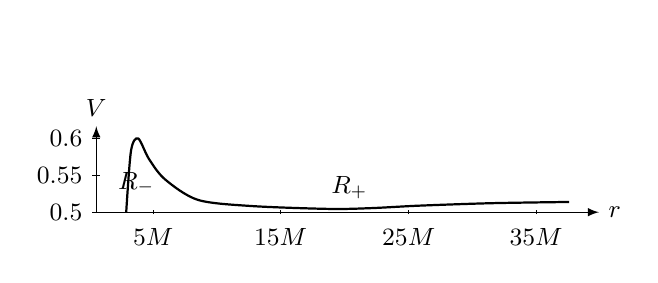
\begin{tikzpicture}[x=.76cm,y=5.2cm,>=latex,font=\small]
  \draw[->] (0,.46) -- (8.4,.46) node[right] {\(r\)};
  \draw[->] (0,.46) -- (0,.67) node[above] {\(V\)};
  \foreach \x/\lab in {.95/\(5M\),3.08/\(15M\),5.22/\(25M\),7.35/\(35M\)}
    \draw (\x,.455) -- (\x,.465) node[below=3pt] {\lab};
  \foreach \y/\lab in {.46/0.5,.55/0.55,.64/0.6}
    \draw (-.07,\y) -- (.07,\y) node[left=3pt] {\lab};
  \draw[thick,smooth] plot coordinates {
    (.50,.46) (.58,.61) (.70,.64) (.88,.59) (1.15,.54) (1.7,.49)
    (2.6,.475) (3.9,.468) (4.6,.470) (5.4,.476) (6.6,.482) (7.9,.485)};
  \node[above=3pt] at (.67,.46) {\(R_-\)};
  \node[above] at (4.23,.47) {\(R_+\)};
  % Reserve trim clearance above the artwork when this float lands at page top.
  \path[draw=none] (0,.91) circle[radius=.1pt];
\end{tikzpicture}
\caption{The effective potential, \(V\), for timelike geodesics in the case
\(L^2=24M^2\). (Note that the scale of \(V\) is greatly expanded as compared
with Figure~\ref{fig:6.3}.)}
\label{fig:6.4}
\end{figure}
\endgroup


The energy of an ordinary particle in one-dimensional motion which sits at the
minimum or maximum of a potential \(V\) is, of course, just the value of \(V\) at
that point. Thus, from our mathematical analogy, Eq.~\eqref{eq:6.3.14}, we see
that the true energy per unit rest mass, \(E\), of a particle in a circular orbit
of radius \(R\) is given by
\begin{equation}
  \frac12E^2(R)=V(R)=\frac12\frac{(R-2M)^2}{R(R-3M)},
  \tag{6.3.21}\label{eq:6.3.21}
\end{equation}
so that
\begin{equation}
  E(R)=\frac{R-2M}{R^{1/2}(R-3M)^{1/2}},
  \tag{6.3.22}\label{eq:6.3.22}
\end{equation}
where Eq.~\eqref{eq:6.3.16} was used to eliminate \(L^2\) in terms of \(R\)
(= \(R_+\) or \(R_-\)). Note that if \(R\leq4M\), we have \(E\geq1\) and,
indeed, \(E\to\infty\) as \(R\to3M\). Thus, particles in the unstable circular
orbits between \(3M\) and \(4M\) would escape to infinity if perturbed radially
outward.

The binding energy, \(E_B\), per unit rest mass of the last stable circular orbit
at \(R=6M\) is
\begin{equation}
  E_B=1-E=1-(8/9)^{1/2}\approx0.06.
  \tag{6.3.23}\label{eq:6.3.23}
\end{equation}

Now, a particle orbiting in the Schwarzschild geometry will emit gravitational
radiation, as discussed for weak fields in Section~4.4b. Because of radiation
reaction, it will deviate slightly from geodesic motion. A particle initially in a
circular orbit with \(R\gg M\) (and thus with \(E\approx1\)) should slowly spiral
in to smaller radii as it loses energy by gravitational radiation, remaining in a
nearly circular orbit until it reaches the orbital radius \(R=6M\). At that point,
the orbit becomes unstable and the particle should rapidly fall to \(r=0\).
According to Eq.~\eqref{eq:6.3.23}, about \(6\%\) of the original mass-energy of
the particle will be radiated away during the time in which the particle spirals
to \(R=6M\). (For the Kerr metric with \(a=M\), the corresponding fraction of
energy radiated is \(42\%\); see Chapter~12.) This illustrates that although the
emission of gravitational radiation was found to be very weak in the examples of
Section~4.4b, large amounts of energy can be converted to gravitational radiation
in astrophysically plausible processes.

If a particle is displaced slightly from the equilibrium radius \(R_+\) of a
stable circular orbit, the particle will oscillate in radius about \(R_+\). For
sufficiently small displacements, it will execute simple harmonic motion with
frequency \(\omega_r\), given by
\begin{equation}
  \omega_r^2=k_{\mathrm{eff}}
  =\left.\frac{d^2V}{dr^2}\right|_{R_+}
  =\frac{M(R_+-6M)}{R_+^3(R_+-3M)},
  \tag{6.3.24}\label{eq:6.3.24}
\end{equation}
where Eq.~\eqref{eq:6.3.16} was used to eliminate \(L^2\), and we should
emphasize that the time implicit in \(\omega_r\) is the proper time \(\tau\)
measured by the particle as opposed to the coordinate time \(t\) of the
Schwarzschild geometry. On the other hand, for a circular orbit, the angular
frequency, \(\omega_\phi=\dot\phi\), is given by Eq.~\eqref{eq:6.3.13},
\begin{equation}
  \omega_\phi^2=\frac{L^2}{R_+^4}=\frac{M}{R_+^2(R_+-3M)},
  \tag{6.3.25}\label{eq:6.3.25}
\end{equation}
where, again, Eq.~\eqref{eq:6.3.16} was used to eliminate \(L^2\). In the limit
of Newtonian orbits, \(R_+\gg M\), we have \(\omega_r\approx\omega_\phi\). If
\(\omega_r=\omega_\phi\), then the particle would return to a given value of \(r\)
exactly one orbital period later; i.e., the orbit will close. Indeed, in the
Newtonian theory of gravity, all bound orbits---not just the nearly circular
orbits---are closed ellipses. The failure of \(\omega_r\) to equal
\(\omega_\phi\) in general relativity means that the orbits do not close; rather
there is a precession of the angle at which the maximum and minimum values of
\(r\) are achieved. For nearly circular orbits, this precession rate is given by
\begin{equation}
  \omega_p=\omega_\phi-\omega_r
  =-\left[(1-6M/R_+)^{1/2}-1\right]\omega_\phi.
  \tag{6.3.26}\label{eq:6.3.26}
\end{equation}
In the limit \(R_+\gg M\), we have, to lowest nonvanishing order,
\begin{equation}
  \omega_p\approx\frac{3M^{3/2}}{R_+^{5/2}}
  =\frac{3(GM)^{3/2}}{c^2R_+^{5/2}},
  \tag{6.3.27}\label{eq:6.3.27}
\end{equation}
where we have restored the \(G\)'s and \(c\)'s in the final formula. We have
considered only nearly circular orbits here, but a more general analysis (see,
e.g., Weinberg 1972) shows that to lowest nonvanishing order the precession of an
arbitrary elliptical orbit is given by
\begin{equation}
  \omega_p\approx\frac{3(GM)^{3/2}}{c^2(1-e^2)a^{5/2}},
  \tag{6.3.28}\label{eq:6.3.28}
\end{equation}
where \(a\) is the semimajor axis of the ellipse and \(e\) is its eccentricity.
For the orbit of the planet Mercury, general relativity predicts a precession rate
of 43 seconds of arc per century. Precisely this residual precession rate had been
observed (after taking into account known effects such as perturbations of the
planet Venus) prior to the formulation of general relativity and had been an
unexplained mystery. The explanation of the precession of Mercury's orbit by
general relativity was one of the most dramatic early successes of the theory.
Although the general relativistic precession of Mercury's orbit is extremely
small, the similar precession observed in the orbit of the binary pulsar mentioned
at the end of Chapter~4 is about \(4^\circ\) per year. This result has been used
to estimate the masses of the two bodies in this system.

We turn, now, to consideration of the null geodesics. Setting \(\kappa=0\) in
Eq.~\eqref{eq:6.3.14}, we find the effective potential for null geodesics to be
simply
\begin{equation}
  V=\frac{L^2}{2r^3}(r-2M).
  \tag{6.3.29}\label{eq:6.3.29}
\end{equation}
Thus, the shape of \(V\) is independent of \(L\) and, as illustrated in
Figure~\ref{fig:6.5}, the only extremum of \(V\) is a maximum occurring at
\(r=3M\). Thus, in general relativity, unstable circular orbits of photons exist
at radius \(3M\), so that, physically, gravity has a very significant effect on
the propagation of light rays in the strong field regime.
% Source: Wald GR, physical PDF p. 156
%         (printed p. 143).
% Coverage: Figure 6.5, effective potential for null geodesics.
% Figures/tables/footnotes: Figure 6.5; no tables or footnotes.
% Status: source-reviewed and compile-clean.
% Uncertainties: none.
\begingroup
\renewcommand{\thefigure}{6.5}
\begin{figure}[htbp]
\centering
\begin{tikzpicture}[x=.75cm,y=1.45cm,>=latex,font=\small]
  \draw[->] (0,0) -- (8.1,0) node[right] {\(r\)};
  \draw[->] (0,-1.45) -- (0,1.95) node[above] {\(V\)};
  \foreach \x/\lab in {1.25/\(3M\),2.1/\(5M\),4.25/\(10M\),6.4/\(15M\)}
    \draw (\x,.06) -- (\x,-.06) node[below=3pt] {\lab};
  \node[left] at (0,0) {0};
  \draw[thick,smooth] plot coordinates {
    (.82,-1.35) (.94,-.30) (1.13,.72) (1.36,1.12) (1.62,.93)
    (2.2,.62) (3.1,.34) (4.3,.18) (5.6,.10) (7.55,.045)};
\end{tikzpicture}
\caption{The effective potential, \(V\), for null geodesics.}
\label{fig:6.5}
\end{figure}
\endgroup

The minimum energy, \(E\), required to surmount the top of the potential barrier
is given by (see Eq.~\eqref{eq:6.3.21} above)
\begin{equation}
  \frac12E^2=V(R=3M)=\frac{L^2M}{2(3M)^3},
  \tag{6.3.30}\label{eq:6.3.30}
\end{equation}
i.e.,
\begin{equation}
  L^2/E^2=27M^2.
  \tag{6.3.31}\label{eq:6.3.31}
\end{equation}
Now, for a light ray propagating in flat spacetime, it follows directly from the
definitions of \(L\) and \(E\) that \(L/E\) is the impact parameter of the light
ray, i.e., the distance of closest approach to the origin \(r=0\). Since the
Schwarzschild geometry is asymptotically flat, for a light ray initially in the
asymptotically flat region (\(r\gg M\)), \(L/E\) will represent the \emph{apparent
impact parameter},
\begin{equation}
  b\equiv L/E,
  \tag{6.3.32}\label{eq:6.3.32}
\end{equation}
of the light ray even though it no longer represents the distance of closest
approach. Thus, the Schwarzschild geometry will capture any photon sent toward it
with an apparent impact parameter smaller than the critical value, \(b_c\), given
by
\begin{equation}
  b_c=3^{3/2}M.
  \tag{6.3.33}\label{eq:6.3.33}
\end{equation}
Hence, the capture cross section, \(\sigma\), for photons in the Schwarzschild
geometry is
\begin{equation}
  \sigma=\pi b_c^2=27\pi M^2.
  \tag{6.3.34}\label{eq:6.3.34}
\end{equation}

To analyze the light bending effects of the Schwarzschild geometry on the light
rays which are not captured, it is convenient to derive an equation for the
spatial orbit of the light ray by solving Eq.~\eqref{eq:6.3.14} for \(\dot r\) and
then dividing \(\dot\phi\), Eq.~\eqref{eq:6.3.13}, by \(\dot r\). We obtain
\begin{equation}
  \frac{d\phi}{dr}=\frac{L}{r^2}
  \left[E^2-\frac{L^2}{r^3}(r-2M)\right]^{-1/2}.
  \tag{6.3.35}\label{eq:6.3.35}
\end{equation}
We wish to find the change, \(\Delta\phi=\phi_{+\infty}-\phi_{-\infty}\), in the
angular coordinate \(\phi\) of a light ray in the Schwarzschild geometry
traversing a path as illustrated in Figure~\ref{fig:6.6}. In order not to be
captured, the impact parameter, \(b\), must be greater than the critical value,
Eq.~\eqref{eq:6.3.33}. In that case, the orbit of the light ray will have a
turning point at the largest radius, \(R_0\), for which \(V(R_0)=E^2/2\), i.e.,
at the largest root of
% Source: Wald GR, physical PDF p. 157
%         (printed p. 144).
% Coverage: Figure 6.6, bending of light.
% Figures/tables/footnotes: Figure 6.6; no tables or footnotes.
% Status: source-reviewed and compile-clean.
% Uncertainties: none.
\begingroup
\renewcommand{\thefigure}{6.6}
\begin{figure}[htbp]
\centering
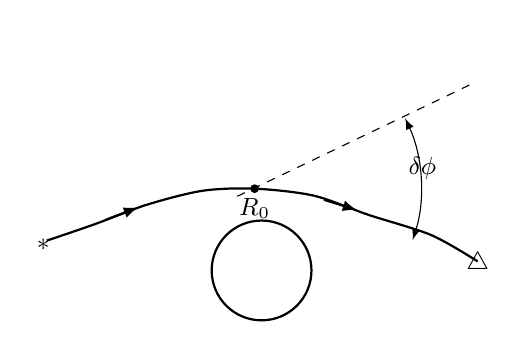
\begin{tikzpicture}[scale=.88,>=latex,font=\small]
  \draw[thick] (0,-.35) circle (.72);
  % Tangent to the ray at closest approach; its angular separation from the
  % outgoing asymptote is the deflection angle.
  \draw[dashed] (-.35,.72) -- (3.05,2.35);
  \draw[thick,smooth] plot coordinates {
    (-3.1,.08) (-2.4,.32) (-1.65,.60) (-.85,.80) (-.10,.83)
    (.75,.73) (1.55,.45) (2.45,.16) (3.12,-.22)};
  \draw[->,thick] (-2.25,.38) -- (-1.78,.56);
  \draw[->,thick] (.90,.67) -- (1.38,.52);
  \fill (-.10,.83) circle (1.8pt) node[below] {\(R_0\)};
  \node at (-3.15,.02) {\(\ast\)};
  \node at (3.12,-.24) {\(\triangle\)};
  \draw[<->] (2.18,.09) arc[start angle=-18,end angle=25,radius=2.40];
  \node at (2.32,1.12) {\(\delta\phi\)};
  % Reserve trim clearance above the artwork when this float lands at page top.
  \path[draw=none] (0,3.15) circle[radius=.1pt];
\end{tikzpicture}
\caption{Diagram illustrating the bending of light effect.}
\label{fig:6.6}
\end{figure}
\endgroup

\begin{equation}
  R_0^3-b^2(R_0-2M)=0,
  \tag{6.3.36}\label{eq:6.3.36}
\end{equation}
which is
\begin{equation}
  R_0=\frac{2b}{\sqrt3}
  \cos\left[\frac13\cos^{-1}\left(-\frac{3^{3/2}M}{b}\right)\right].
  \tag{6.3.37}\label{eq:6.3.37}
\end{equation}
By symmetry, the contributions to \(\Delta\phi\) made by the parts of the path
prior to the turning point and after the turning point will be equal. Hence, by
Eq.~\eqref{eq:6.3.35}, the total change in the angular coordinate,
\(\Delta\phi\), is given by
\begin{equation}
  \Delta\phi=2\int_{R_0}^{\infty}
  \frac{dr}{[r^4b^{-2}-r(r-2M)]^{1/2}}.
  \tag{6.3.38}\label{eq:6.3.38}
\end{equation}
It is convenient to make the change of variables, \(u=1/r\), in terms of which
Eq.~\eqref{eq:6.3.38} becomes
\begin{equation}
  \Delta\phi=2\int_0^{1/R_0}
  \frac{du}{(b^{-2}-u^2+2Mu^3)^{1/2}}.
  \tag{6.3.39}\label{eq:6.3.39}
\end{equation}
In the case of flat spacetime, \(M=0\), we have \(R_0=b\), and
Eq.~\eqref{eq:6.3.39} yields simply
\begin{equation}
  \left.\Delta\phi\right|_{M=0}=2\sin^{-1}(b/R_0)=\pi,
  \tag{6.3.40}\label{eq:6.3.40}
\end{equation}
as obviously must be the case since the trajectory is a straight line. When
\(M\ne0\), according to Eq.~\eqref{eq:6.3.39} \(\Delta\phi\) will not equal
\(\pi\); i.e., there will be a nonzero deflection of the light ray, which we may
interpret physically as being due to the gravitational attraction of the
Schwarzschild geometry. We wish to calculate the contribution to the light
bending valid to first order in \(M\). Actually, it is rather tricky to calculate
this contribution by varying \(M\) keeping \(b\) fixed in Eq.~\eqref{eq:6.3.39}
because of the \(M\) dependence of the integration limit \(1/R_0\) and the
singular behavior of the integrand at this limit. However, we can circumvent these
difficulties by working with \(M\) and \(R_0\) as the independent variables. In
other words, as we vary \(M\), we compare \(\Delta\phi\) for light rays which
have the same Schwarzschild radial coordinate, \(R_0\), at the point of closest
approach rather than, say, light rays with the same apparent impact parameter,
\(b\). (It is not difficult to see that to first order in \(M\), it makes no
difference whether we keep \(b\) or \(R_0\) fixed, but to higher orders in \(M\)
it \emph{does} matter whether we compare light rays with the same value of \(b\)
or the same value of \(R_0\).) Eliminating \(b\) via Eq.~\eqref{eq:6.3.36}, we
obtain
\begin{equation}
  \Delta\phi=2\int_0^{1/R_0}
  \frac{du}{(R_0^{-2}-2MR_0^{-3}-u^2+2Mu^3)^{1/2}}.
  \tag{6.3.41}\label{eq:6.3.41}
\end{equation}
Differentiating with respect to \(M\) at fixed \(R_0\) and evaluating the result
at \(M=0\), we obtain
\begin{align}
  \left.\frac{\partial(\Delta\phi)}{\partial M}\right|_{M=0}
    &=2\left.\int_0^{1/R_0}
       \frac{(R_0^{-3}-u^3)\,du}
       {(R_0^{-2}-2MR_0^{-3}-u^2+2Mu^3)^{3/2}}\right|_{M=0}\nonumber\\
    &=2\int_0^{1/b}\frac{(b^{-3}-u^3)\,du}{(b^{-2}-u^2)^{3/2}}
      =4b^{-1}.
  &&\tag{6.3.42}\label{eq:6.3.42}
\end{align}
Thus, to first order in \(M\), the deflection of light is given by
\begin{align}
  \delta\phi
    &=\Delta\phi-\pi
      \approx M\left.\frac{\partial(\Delta\phi)}{\partial M}\right|_{M=0}
      =\frac{4M}{b}\nonumber\\
    &=\frac{4GM}{bc^2},
  &&\tag{6.3.43}\label{eq:6.3.43}
\end{align}
where we have reinserted the \(G\)'s and \(c\)'s in the last step. For a light
ray which grazes the surface of the Sun, Eq.~\eqref{eq:6.3.43} predicts a
deflection of \(1.75\) seconds of arc. This bending of starlight passing near the
Sun has been observed during solar eclipses beginning with the 1919 expedition led
by Eddington (Dyson, Eddington, and Davidson 1920), thus confirming this important
prediction of general relativity, but because of numerous difficulties the
accuracy of these measurements has only been about \(10\%\). However, the bending
of radio waves emitted from a quasar as it approaches eclipse by the Sun has been
measured to about \(1\%\) accuracy (Fomalont and Sramek 1976) and has been found
to agree with Eq.~\eqref{eq:6.3.43}.

A further measurable effect concerning the behavior of null geodesics in the
Schwarzschild geometry is the time delay of radar signals emitted from Earth. To
analyze this effect, we divide \(t\), as given by Eq.~\eqref{eq:6.3.12}, by
\(\dot r\), as determined from Eq.~\eqref{eq:6.3.14}, thereby obtaining
\begin{equation}
  \frac{dt}{dr}=\left(1-\frac{2M}{r}\right)^{-1}
  \left[1-\left(1-\frac{2M}{r}\right)\frac{b^2}{r^2}\right]^{-1/2}.
  \tag{6.3.44}\label{eq:6.3.44}
\end{equation}
Integration of this equation over the trajectory of a null geodesic yields the
total change, \(\Delta t\), in Schwarzschild time coordinate along the
trajectory. Consider, now, the following situation. A radar signal is emitted
from Earth, located at Schwarzschild radial coordinate \(R_E\). The signal passes
near the Sun, with radius of closest approach \(R_0\), and then is reflected off a
planet, located at \(R_P\). The signal then retraces its trajectory and returns to
Earth, as illustrated in Figure~\ref{fig:6.7}. (The motion of Earth and the planet
during the intervening time is neglected.) How much time, \(\Delta\tau\), elapses
on the clock of an observer on Earth between emission and reception of the signal?
We wish to calculate \(\Delta\tau\) to first order in \(M\). By integrating
Eq.~\eqref{eq:6.3.44} and then differentiating with respect to \(M\) (holding
\(R_0\) fixed) we obtain (problem~5), in close analogy to the derivation of the
light bending effect,
\begin{align}
  \Delta t=\frac{2}{c}\biggl\{
    &(R_E^2-R_0^2)^{1/2}+(R_P^2-R_0^2)^{1/2}\nonumber\\
    &+\frac{2GM}{c^2}\biggl[
      2\ln\left(\frac{R_E+(R_E^2-R_0^2)^{1/2}}{R_0}\right)
      +2\ln\left(\frac{R_P+(R_P^2-R_0^2)^{1/2}}{R_0}\right)\nonumber\\
    &\qquad\quad+\left(\frac{R_E-R_0}{R_E+R_0}\right)^{1/2}
      +\left(\frac{R_P-R_0}{R_P+R_0}\right)^{1/2}
    \biggr]\biggr\}.
  &&\tag{6.3.45}\label{eq:6.3.45}
\end{align}
% Source: Wald GR, physical PDF p. 160
%         (printed p. 147).
% Coverage: Figure 6.7, time delay of light.
% Figures/tables/footnotes: Figure 6.7; no tables or footnotes.
% Status: source-reviewed and compile-clean.
% Uncertainties: none.
\begingroup
\renewcommand{\thefigure}{6.7}
\begin{figure}[htbp]
\centering
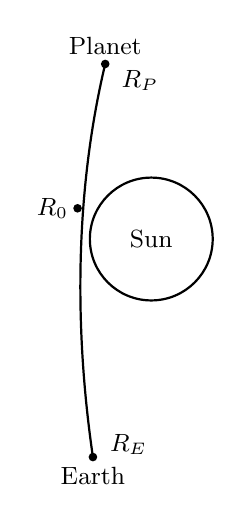
\begin{tikzpicture}[scale=.78,>=latex,font=\small]
  \draw[thick] (.7,.2) circle (1.0);
  \node at (.7,.2) {Sun};
  \draw[thick] (-.25,-3.35) .. controls (-.55,-1.3) and (-.55,.95) .. (-.05,3.05);
  \fill (-.25,-3.35) circle (2pt) node[below] {Earth};
  \node[right] at (-.13,-3.15) {\(R_E\)};
  \fill (-.50,.70) circle (2pt) node[left] {\(R_0\)};
  \fill (-.05,3.05) circle (2pt) node[above] {Planet};
  \node[right] at (.06,2.78) {\(R_P\)};
\end{tikzpicture}
\caption{Diagram illustrating the time delay of light effect.}
\label{fig:6.7}
\end{figure}
\endgroup

It should be noted that we have formulated the question purely for mathematical
convenience, so that as we vary \(M\), we compare null geodesics with the same
\(R_0\), rather than, say, null geodesics with the same \(b\) or the same total
change, \(\Delta\phi\), in angle in passing between \(R_E\) and \(R_P\). Unlike
the light bending case, here the first order terms in \(M\) depend sensitively on
what parameters of the null geodesics are held fixed as \(M\) is varied.

The proper time, \(\Delta\tau\), that elapses on Earth is related to the change in
coordinate time, \(\Delta t\), by
\begin{equation}
  \Delta\tau=(1-2M/R_E)^{1/2}\Delta t.
  \tag{6.3.46}\label{eq:6.3.46}
\end{equation}
Thus, to first order in \(M\), the reflected radar signal will be measured to
arrive back on Earth at a time after emission given by
\begin{equation}
  \Delta\tau=-\frac{2GM}{c^3R_E}
  \left[(R_E^2-R_0^2)^{1/2}+(R_P^2-R_0^2)^{1/2}\right]+\Delta t,
  \tag{6.3.47}\label{eq:6.3.47}
\end{equation}
where \(\Delta t\) is given by Eq.~\eqref{eq:6.3.45}.

Actually, Eq.~\eqref{eq:6.3.47} by itself is not very useful for a direct test
of the general relativistic time delay effect, since the parameters \(R_E\),
\(R_P\), and \(R_0\) appearing in the equation are not known to the necessary
precision. Therefore, the procedure used to test the time delay prediction is to
write down a formula for how \(\Delta\tau\) is expected to vary with time (due to
the motion of the Earth and planets), treating all parameters (in particular, the
orbital parameters of the planets) as unknowns. A best fit to the observed data
then is used to determine all the parameters. When this is done, the agreement
between the theoretical formula and observation is excellent. On the other hand, a
slight modification of the general relativistic contribution---in particular, the
change that would be produced in the formula by altering \(g_{rr}\) to
\((1-2\gamma M/r)^{-1}\), where \(\gamma\) differs from unity by only
\(0.2\%\)---produces a formula which cannot be satisfactorily fit by the observed
data. (These highest precision data actually have come from the tracking of
spacecraft which emit signals rather than reflection of radar off of planets
[Reasenberg \emph{et al.}\ 1979].) Thus, this prediction of general relativity
has been confirmed to high precision.

In summary, the analysis of timelike and null geodesics in the Schwarzschild
geometry leads to a number of important predictions which have been tested by
solar system observations: the gravitational redshift, the precession of planetary
orbits, the bending of light, and the time delay of radar signals. These
predictions provide stringent quantitative tests of general relativity, and it is
gratifying that general relativity thus far has passed these tests very
successfully.
